\section{Conclusion}
\label{sec:conclusion}

In this laboratory assignment the objective of building a bandpass filter with central frequency at aproximately 1kHz and gain at central frequency $40dB$ was achieved. The central frequency was $1006.5 Hz$, so it presents a deviation of only $0.65 \%$.
The maximum obtained was $36.55dB$, which presents a deviation of $8.6 \%$. The cost was $113.44$ MU and the merit was $3.9375\cdot 10^{-4}$
 
The results from both the physical circuit at the laboratory and the circuit
simulation using ngspice appear to match, as we can see in the following figure:



\begin{minipage}[c]{0.50\linewidth}
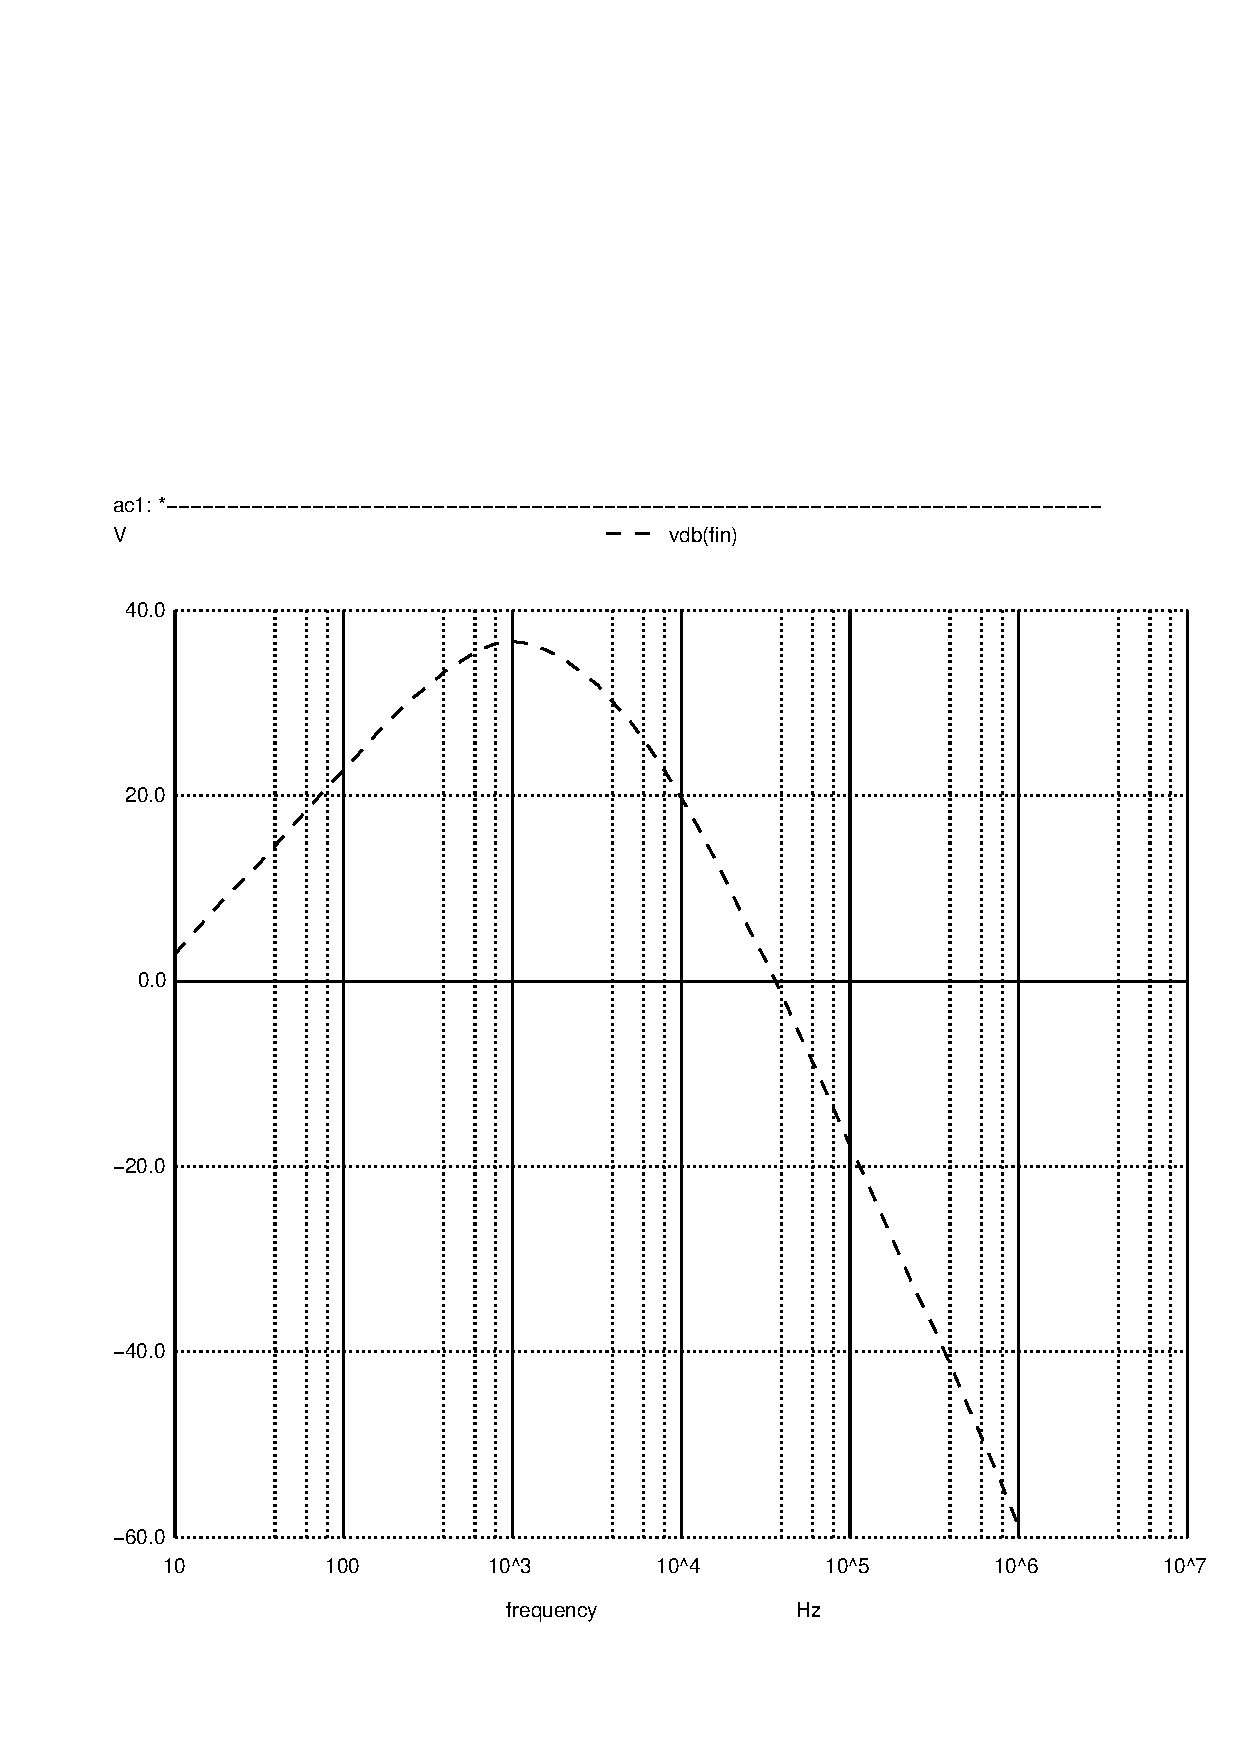
\includegraphics[width=1\linewidth]{../sim/vo1f.pdf}
\end{minipage} % no space if you would like to put them side by side
\hspace{1mm}
\begin{minipage}[c]{0.50\linewidth}
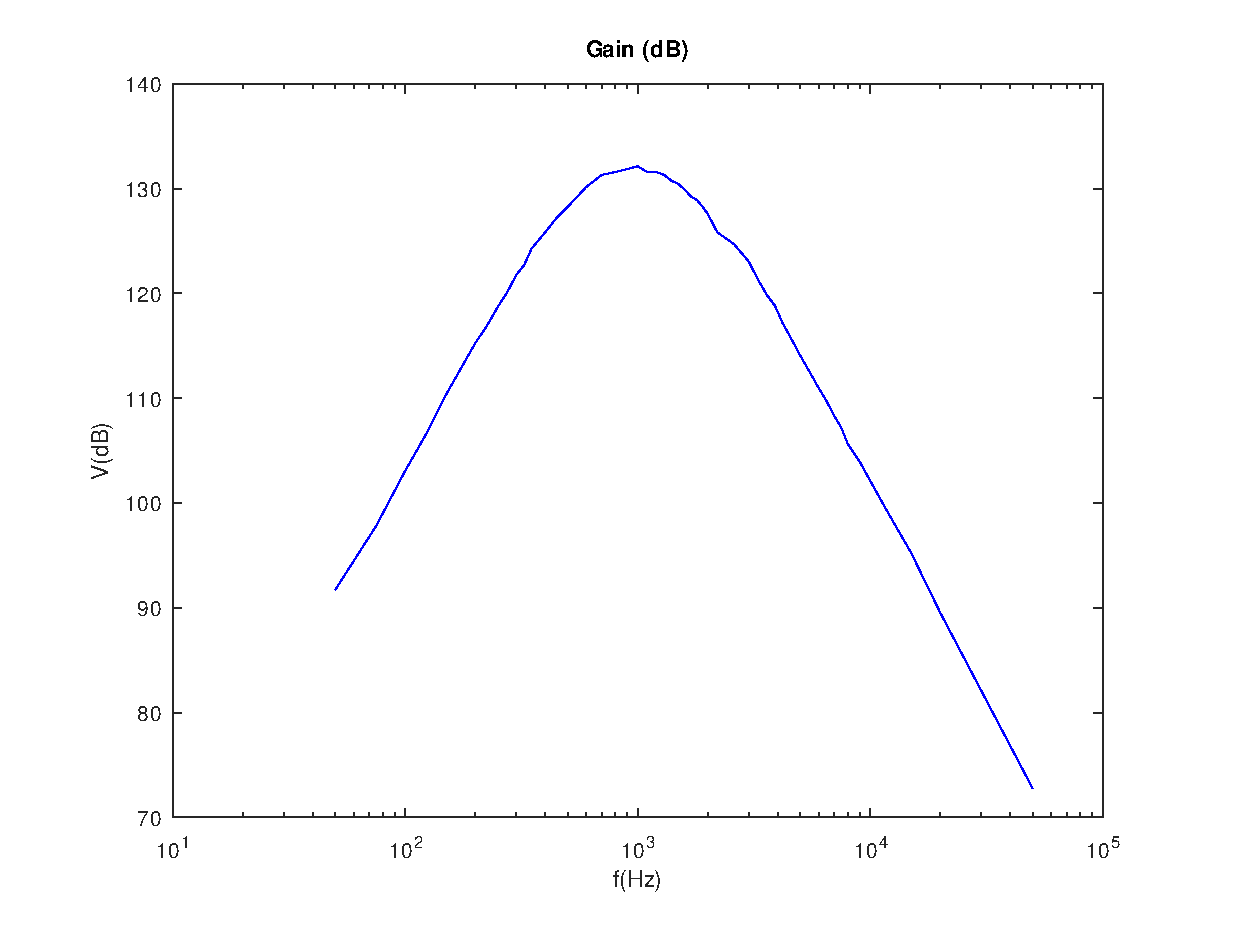
\includegraphics[width=1\linewidth]{lab.eps}
\end{minipage}


\par
We can conclude that the physical circuit and simulation analysis yield very similar results.
However, the theoretical analysis yielded very lacklustre values. This is probably due to the complexity of the OP-AMP component which the simple model used failed to replicate.